\documentclass[a4paper,11pt,aps,final]{revtex4}

\usepackage[utf8x]{inputenc}
\usepackage[dvips]{graphicx}
\usepackage{hyperref}

\begin{document}

\title{How to use the \textsf{multilayers} \textsf{Python} module}
\author{Joan Juvert}
\email{joan.juvert@imb-cnm.csic.es}
\affiliation{Institut de Microelectrònica de Barcelona, CNM-CSIC, Campus UAB, 08193 Bellaterra, Spain}

\begin{abstract}

This tutorial will get you started with the use of the \textsf{multilayers} \textsf{Python} module. You will learn how to set up your multilayered system and how to extract some of its optical charactersitics.

\end{abstract}

\maketitle

\section{Introduction}

The \textsf{multilayers} \textsf{Python} module allows you to calculate the effect of a multilayered system on the propagation of light. In particular, you will be able to calculate the characteristic matrices of the whole system or any of its layers, the reflection and transmission coefficients, the reflectance and transmittance\cite{born00}.

Furthermore, consider a radiative center at some point of the multilayered system whose emission is detected by an observer at infinity. The \textsf{multilayers} module will allow the user to calculate the ratio of the energy detected by the observer in the presence of the multilayer to the energy he would receive if there was no multilayer (i.e. if the whole system was made of the same medium the observer is standing on). In order to calculate this, the module makes use of a method developed by O. H. Crawford and published in ref. \onlinecite{crawford88}.

\section{Dependencies}

In this section you will find what you need to have in order to use the \textsf{multilayers} module.

\subsection{\textsf{Python}}

You will need \textsf{Python} to use the \textsf{multilayers.py} module. In the web page\cite{python} you will find links to installers for all major operating systems. Linux users can just install it from the package manager of their distribution.

To follow this tutorial it is not strictly necessary to know \textsf{Python} because the syntax of the statements we will use is very straightforward. However, a basic knowledge of some programming language is required in order to at least grasp the idea of what we're doing.

\subsection{\textsf{Numpy}}

\textsf{Numpy} is a \textsf{Python} module that provides a suitable array type for numerical calculations. In the web page\cite{numpy} you can find installers for all major operating systems. As with \textsf{Python}, Linux users can get it from their package manager.

\subsection{\textsf{Scipy}}

\textsf{Scipy} is a \textsf{Python} module for mathematics, science and engineering. As with \textsf{Numpy}, in the web page\cite{scipy} you can find installers for all major operating systems. Linux users can get it from their package manager.

\subsection{\textsf{Git}}

\textsf{Git} is a version control system. You will need this to get the \textsf{multilayers} module from \textsf{github}\cite{github}. You can find installers for all major operating systems on the web\cite{git}. Linux users can get it from their package manager.

\section{Installation}

To install the multilayers module you just have to clone it from a public repository in \textsf{github}\cite{github}. If you already have git installed, cloning the repository is as easy as typing:

\begin{verbatim}
    joan@pc6183:~$ git clone git://github.com/tortugueta/multilayers.git
\end{verbatim}

That will create a \texttt{multilayers} directory and store all the files of the project inside. See the file \texttt{README.md} to learn more about the contents of the project.

\section{Usage}

Here you will learn how to use the \textsf{multilayers} module.

Before you begin, if you plan to work in a directory other than \texttt{multilayers} (which is most likely) you will need to add that directory to your \texttt{PYTHONPATH} environment variable. In \textsf{Bash} you can do this by typing:

\begin{verbatim}
    joan@pc6183:~$ PYTHONPATH=${PYTHONPATH}:/home/user/multilayers
\end{verbatim}

Replace \texttt{/home/user/multilayers} for the appropiate directory. This will allow you to import the \textsf{multilayers} module even if you are not in the directory where \textsf{multlayers.py} is located. If you want to make this change permanent, add that line in the \texttt{.bashrc} file located in your home directory.

Now you can start by launching the \textsf{Python} interpreter:

\begin{verbatim}
    joan@pc6183:~$ python
    Python 2.6.6 (r266:84292, Dec 26 2010, 22:31:48)
    [GCC 4.4.5] on linux2
    Type "help", "copyright", "credits" or "license" for more information.
    >>>
\end{verbatim}

You must import the \textsf{multilayers} module before you can use it:

\begin{verbatim}
    >>> import multilayers as ml
    >>>
\end{verbatim}

We will also use \textsf{Numpy} so we will import it as well:

\begin{verbatim}
    >>> import numpy as np
    >>>
\end{verbatim}


\subsection{Defining the mediums}

A medium will be defined by its complex refractive index $\tilde n$, which is a function of the wavelength $\lambda$. From now on, I will use the term \emph{refractive index} to refer to the real part $n$ of the complex refractive index $\tilde n$. The term \emph{extintion coefficient} will be used to refer to the imaginary part $k$ of the complex refractive index $\tilde n$.

In order to define a medium, you will need a plain text file with three columns: one for the wavelength, another for the refractive index $n$ and a third for the extintion coefficient $k$. In the \texttt{examples} subdirectory of the \textsf{multilayers} directory you can find example files for air, silicon, silicon dioxide, silicon nitride and polysilicon.

To load a medium just type:

\begin{verbatim}
    >>> dielectric = ml.Medium("examples/sio2.dat")
    >>>
\end{verbatim}

Here what we do is load the table of refractive indices of the file \texttt{examples/sio2.dat}. Replace that for the path to the file you want to use. This creates a \texttt{Medium} object and we assign this object to a variable called \texttt{dielectric}.

If your file has more columns than necessary, they are in an order other than $(\lambda\;n\;k)$, they are separated by characters other than \texttt{TAB} or the comments start by something other than \texttt{\#}, you can pass some options to the previous call that will allow you to tweak the loading of the table. See the reference to the \texttt{Medium} class for more information about that.

Once we have the medium loaded, we can do a number of things with it. First, note that even though your file has the refractive indices sampled at a discrete number of wavelengths, you can get the complex refractive index at any wavelength within the range defined by the maximum and minimum wavelengths of your sampling. That is because the program builds an interpolator with the provided data. This is important because that frees you of the necessity to make sure that all your materials are sampled at precisely the same wavelengths.

To recover the range where you can interpolate the refractive index, just type:

\begin{verbatim}
    >>> dielectric.getMinMaxWlength()
    (160.0, 2500.0)
    >>>
\end{verbatim}

You can check that 160.0 nm and 2500.0 nm are the minimum and maximum wavelengths in the file \texttt{examples/sio2.dat}.

To find out the complex refractive index at any wavelength within the interpolable range, for instance 502 nm, type:

\begin{verbatim}
    >>> dielectric.getRefrIndex(502)
    (1.4622175947399658+0j)
    >>>
\end{verbatim}

Notice that we get the complex refractive index, altough in this case the extintion coefficient is zero. Also, notice that the interpolating function passes through the sampled points, which means that you can recover exactly the values at the sampled wavelengths (within the roundoff error)

\begin{verbatim}
    >>> dielectric.getRefrIndex(500)
    (1.4622999999999993+0j)
    >>>
\end{verbatim}

You can check in the \texttt{examples/sio2.dat} file that the value of the refractive index at 500 nm is 1.4623.

The units of the wavelength in your files may be anything, but you have to be consistent during the program and use always the same units.

\subsection{Defining the multilayer system} \label{sub:define_multilayer}

Before building our multilayer system, let's load two more materials.

\begin{verbatim}
    >>> air = ml.Medium("examples/air.dat")
    >>> substrate = ml.Medium("examples/silicon.dat")
    >>>
\end{verbatim}

Now we want to work with a simple multilayer system consisting of a dielectric layer 300 nm thick on top of a silicon substrate. The medium above the layer will be air\footnote{Here we will consider the silicon substrate to be a semiinfinite medium just like the air above the dielectric. Since typically the substrate will be much thicker than the layer, it is fine to make that approximation. We could also define the layer strictly and consider the silicon substrate to be a layer of finite thickness and use another layer of air as the bottom medium instead of the silicon.}. See figure \ref{fig:diagram}. We can generate the \texttt{Multilayer} object as follows:

\begin{verbatim}
    >>> multilayer = ml.Multilayer([
    ...         air,
    ...         [dielectric, 300],
    ...         substrate])
    >>>
\end{verbatim}

You can type the whole thing in a single line, but typing it like we just did makes the structure that we are creating more visually apparent. We have a \emph{top medium} made of air, then a 300 nm thick layer of dielectric, and a silicon substrate (that we will also refer to as \emph{bottom medium}). We have assigned the newly created \texttt{Multilayer} object to a variable called \texttt{multilayer}.

\textbf{Important!} Note that the thickness must be in the same units as the wavelengths.

\subsection{Setting the state of the system}

Before we can calculate anything, we have to set the state of the system, i.e. the wavelength of the light propagating across the sytem, the angle of propagation and the polarization. Note that setting the wavelength fixes the complex refractive index in effect, and that affects the propagation angles (through Snell's law). Therefore, you must set the wavelength \emph{before} the propagtion angle. The polarization can be set first or last, since it does not affect the other variables.

Set the wavelength to 500 nm with the \texttt{setWlength} method, which gets the wavelength as its only argument:

\begin{verbatim}
    >>> multilayer.setWlength(500)
    >>>
\end{verbatim}

We can check that we are currently working at 500 nm with the \texttt{getWlength} method:

\begin{verbatim}
    >>> multilayer.getWlength()
    500.0
    >>>
\end{verbatim}


Now we can set the propagation angle. The angles are measured with respect to the $z$ axis. So $\theta = 0$ corresponds to propagation perpendicular to the interfaces. What we do is fix the propagation angle in one of the layers of the system with the \texttt{setPropAngle} method, which expects two arguments: the angle in radians and the index of the layer where we are fixing the angle. Each layer in the system is identified by a consecutive index starting with 0 in the top medium. Therefore, in our system the air will have index 0, the dielectric layer index 1, and the silicon substrate index 2.

The propagation angle in the other layers will be automatically calculated according to Snell's law. Here we will be interested in the light that comes out of the system at 25 degrees. Therefore, we will fix the propagation angle to 25 degrees in the top medium (index 0):

\begin{verbatim}
    >>> multilayer.setPropAngle(np.deg2rad(25), 0)
    >>>
\end{verbatim}

Note that the \texttt{setPropAngle} method expects the angle in radians. We can use the \texttt{deg2rad} method in \textsf{Numpy} to convert from degrees to radians. If the index is not specified 0 will be used as a default value.

Now we can check that the propagation angle is correctly set to 25 degrees ($\approx 0.436$ rad) in the top layer and all the other angles have been calculated correctly. We do that with the \texttt{getPropAngle} method, which gets the index of the layer as an argument.

\begin{verbatim}
    >>> multilayer.getPropAngle(0)
    (0.43633231299858238+0j)
    >>> multilayer.getPropAngle(1)
    (0.29319178759065995-0j)
    >>> multilayer.getPropAngle(2)
    (0.09847162694380529-0.0016750238752748126j)
    >>>
\end{verbatim}

Now, notice that the output is always a complex number. Internally, the program always works with complex angles because in some situations the angle \emph{must} be complex, for example when light propagates beyond the critical angle. In layers 0 and 1 we can see that the angle is formally real in the sense that the imaginary part is zero, as it should be. However, in layer 2 (the silicon substrate) the angle has a nonzero imaginary part. That is because in that layer we have a nonzero extintion coefficient. In that kind of medium the propagation angle does not really bear the meaning of a true propagation angle, just like the complex angle we get beyond the critical angle is not really a propagation angle. You can find more on that in ref. \onlinecite{born00}.

Now only the polarization remains to be set. For that, we use the \texttt{setPolarization} method, which gets either \texttt{'te'} or \texttt{'tm'} (case insensitive) as an argument:

\begin{verbatim}
    >>> multilayer.setPolarization('te')
    >>>
\end{verbatim}

We can check the current polarization with the \texttt{getPolarization} method:

\begin{verbatim}
    >>> multilayer.getPolarization()
    'TE'
    >>>
\end{verbatim}

\subsection{Calculating the matrices}

Once we have set the wavelength, propagation angle and polarization, we can calculate the characteristic matrices of each individual layer in the system. We do that with the \texttt{calcMatrices} method, which gets a list with the indices of the layers whose characteristic matrices we want to calculate. An empty list or no argument at all will result in the characteristic matrices of all layers to be calculated.

Since we need all the characteristic matrices, we do:

\begin{verbatim}
    >>> multilayer.calcMatrices()
    >>>
\end{verbatim}

Note that, since the thickness of the top medium and the substrate is infinite, the characteristic matrix does not make sense in those two layers. Therefore, when we instruct the program to calculate the matrices of all the layers as we have just done, in fact it will only calculate the matrices of the intermediate layers (in our case only the silicon dioxide) but not those of the top and bottom mediums.

Now we can see the matrix of each layer if we want. We use the \texttt{getMatrix} method, which gets the index of the layer as its only argument. The matrix of the silicon dioxide layer is:

\begin{verbatim}
    >>> multilayer.getMatrix(1)
    matrix([[ 0.53550286+0.j        ,  0.00000000+0.603282j  ],
            [ 0.00000000+1.18226084j,  0.53550286+0.j        ]])
    >>>
\end{verbatim}

The characteristic matrix of the top and bottom mediums is internally stored as the \texttt{None} value. If we try to print it we get nothing:

\begin{verbatim}
    >>> multilayer.getMatrix(0)
    >>> multilayer.getMatrix(2)
    >>>
\end{verbatim}

Once we have the characteristic matrices of all the individual layers of the system, we are ready to calculate the global characteristic matrix of the multilayered system, which in fact is the matrix product of the matrices of all the layers. We do that with the \texttt{updateCharMatrix} method:

\begin{verbatim}
    >>> multilayer.updateCharMatrix()
    >>>
\end{verbatim}

The \texttt{updateCharMatrix} method calculates two matrices. One corresponding to the propagation in the direction from the top medium to the substrate, and another in the reverse direction. The matrices are in general different since the matrix product is not commutative.

We can see either matrix with the \texttt{getCharMatrixUpDown} and \texttt{getCharMatrixDownUp} methods. The matrix corresponding to propagation from the top medium to the substrate is:

\begin{verbatim}
    >>> multilayer.getCharMatrixUpDown()
    matrix([[ 0.53550286+0.j        ,  0.00000000+0.603282j  ],
            [ 0.00000000+1.18226084j,  0.53550286+0.j        ]])
    >>>
\end{verbatim}

For propagation from the substrate to the top medium we have:

\begin{verbatim}
    >>> multilayer.getCharMatrixDownUp()
    matrix([[ 0.53550286+0.j        ,  0.00000000+0.603282j  ],
        [ 0.00000000+1.18226084j,  0.53550286+0.j        ]])
    >>>
\end{verbatim}

Of course, in this very simple system the characteristic matrix of the whole system is equal to the matrix of its only layer (remember that the top medium and the substrate do not count towards the calculation of the characteristic matrix), and it is trivially the same in both directions too.

\subsection{Getting the coefficients}

When we call the \texttt{updateCharMatrix} method, the program calculates not only the characteristic matrices, but also the reflection and transmission coefficients, the reflectance and the transmittance. To view this values, we use the \texttt{getCoefficientsUpDown} and \texttt{getCoefficientsDownUp}. These methods return a dictionary. The reflection coefficient is stored with the key \texttt{'r'}, the transmission coefficient with the key \texttt{'t'}, the reflectance with \texttt{'R'} and the transmittance with \texttt{'T'}. In the following lines I will store the dictionary in a variable called \texttt{coefUpDown} and then recover each key in different statements:

\begin{verbatim}
    >>> coefUpDown = multilayer.getCoefficientsUpDown()
    >>> coefUpDown['r']
    (-0.053133453578214605+0.47742391532777739j)
    >>> coefUpDown['t']
    (0.24601384152987718-0.32014850303761927j)
    >>> coefUpDown['R']
    0.23075675881605304
    >>> coefUpDown['T']
    (0.76924324118394694+0.01316999164591307j)
    >>>
\end{verbatim}

The reflection and transmission coefficients are always complex numbers because they carry information on the phase of the wave. The reflectance will always be a real number. However, the transmittance may be real or complex. It will be complex whenever we have a complex angle or when the refractive index of either the top or bottom mediums have nonzero extintion coefficient.

In this case, we have a reflectance $R \approx 0.23$, which means that if we have a wave propagating from the air towards the SiO$_2$--on--silicon system, 23\% of the energy will be reflected back towards the air (that is for the wavelength 500 nm and incidence at 25 degrees that we set earlier).

Now we will do the same for the propagation from the silicon towards the SiO$_2$--on--air system. This time we will skip the intermediate step of storing the coefficients in a variable.

\begin{verbatim}
    >>> multilayer.getCoefficientsDownUp()['r']
    (0.45063140231719617-0.14947982025241136j)
    >>> multilayer.getCoefficientsDownUp()['t']
    (1.1867461704360733-1.490830824900075j)
    >>> multilayer.getCoefficientsDownUp()['R']
    0.22541287741705593
    >>> multilayer.getCoefficientsDownUp()['T']
    (0.76924324118394671-0.013169991645913069j)
    >>>
\end{verbatim}

Notice that, although the characteristic matrix was the same for both directions of propagation, the coefficients are not since the system is not at all symmetric (the input and exit mediums are interchanged).

\subsection{Changing the state}

So, we have seen that for TE polarized light with $\lambda = 500$ nm and incidence at 25 degrees from air towards a 300 nm thick silicon dioxide layer on top of silicon substrate the reflectance is 0.23. What if we now want to see what happens when $\lambda = 600$ nm?

Basically, we have to set the state again, following the same order: first the wavelength (because that will change the propagation angles), then the propagation angle and finally the polarization (again, the polarization can be set at the beginning; the only requirement is that if we change the wavelength, we have to set the propagation angles again). In this case, since we want to keep the polarization in TE mode, we don't need to change it.

Every time we change the state we also have to recalculate the characteristic matrices. Therefore, we type:

\begin{verbatim}
    >>> multilayer.setWlength(600)
    >>> multilayer.setPropAngle(np.deg2rad(25), 0)
    >>> multilayer.calcMatrices()
    >>> multilayer.updateCharMatrix()
    >>>
\end{verbatim}

Now let's see how the reflectance has changed:

\begin{verbatim}
    >>> multilayer.getCoefficientsUpDown()['R']
    0.13013272824116065
    >>>
\end{verbatim}

So, at 600 nm the reflectance drops to 13\%.

To finalize this section, let's see how to scan the reflectance of this system for a range of wavelengths, say between $\lambda = 400$ nm and $\lambda = 800$ nm every 50 nm.

\begin{verbatim}
    >>> # Generate the list of wavelengths we want to scan
    >>> wlength_list = np.arange(400, 800 + 50, 50)
    >>>
    >>> # Initialize the array where the results will be stored
    >>> reflectance = np.empty(wlength_list.size)
    >>>
    >>> # Loop over the wavelengths
    >>> for (index, wavelength) in enumerate(wlength_list):
    ...     multilayer.setWlength(wavelength)
    ...     multilayer.setPropAngle(np.deg2rad(25), 0)
    ...     multilayer.calcMatrices()
    ...     multilayer.updateCharMatrix()
    ...     reflectance[index] = multilayer.getCoefficientsUpDown()['R']
    ...
    >>> # Print the results
    >>> reflectance
    array([ 0.49229979,  0.42306659,  0.23075676,  0.09724455,  0.13013273,
            0.22453337,  0.29978883,  0.34321062,  0.360822  ])
\end{verbatim}

\subsection{The $F$ function} \label{sub:ffunction}

In order to understand what the $F$ function is and what is involved in its calculation, have a look at ref. \cite{crawford88}. In short, imagine the layered system we built in section \ref{sub:define_multilayer} and a coordinate system where $z$ is in the direction perpendicular to the interfaces between layers (figure \ref{fig:diagram}).

\begin{figure}
    \centering
    \includegraphics[scale=1,angle=-90]{figure.ps}
    \caption{Schematic view of our layered system}
    \label{fig:diagram}
\end{figure}

Now imagine there is a dipole in $z = z_0$ oscillating along the direction $i,\;i=x,\,y,\,z$ and emitting ligth at wavelength $\lambda$. $F_i(z_0,\, \lambda,\, \theta)$ is the ratio between the electric field that an observer at $z = \infty$ would measure with an angle of incidence $\theta$ with respect to the $z$ axis, to the electric field he would measure if the whole system was the same medium that we have at $\infty$ (in this case air). So, if $F_i(z_0,\, \lambda,\, \theta) = f$ it means that the observer measures an electric field $f$ times what he would measure if there was no layered sytem (everything air).

$F$ is a complex number because it carries information about the phase of the wave. In general we will want to square the modulus of $F$ to get the ratio of the energy rather than the electric field.

The methods \texttt{calculateFx}, \texttt{calculateFy} and \texttt{calculateFz} are used to calculate the $F$ function for dipoles oscillating along the $x$, $y$ and $z$ axis respectively. They receive three arguments: the $z$ coordinate of the dipole, the wavelength of the emitted light, the angle of propagation and the index of the layer where we are fixing the angle (0 if not specified).

When we execute the methods, the state of the system is automatically set according to the arguments. That means that, once we have the multilayer defined as we did in section \ref{sub:define_multilayer}, we can readily execute \texttt{calculateFx}, \texttt{calculateFy} or \texttt{calculateFz} without setting the state. It will be set or changed automatically if necessary. Also, note that \texttt{calculateFy} will set the polarization to TE while \texttt{calculateFx} and \texttt{calculateFz} will set the polarization to TM.

So, for a dipole oscilating along $y$, located at $z_0 = 150$ and considering light at 25 degrees in the air we have:

\begin{verbatim}
    >>> multilayer.calculateFy(150, 500, np.deg2rad(25), 0)
    (0.0044385213156725055+0.68657782956390412j)
    >>>
\end{verbatim}

We are probably more interested in the energy stored in the TE and TM waves. For the TE wave let's calculate $|F_y|^2$, but now for propagation perpendicular to the interfaces:

\begin{verbatim}
    >>> theta = 0
    >>> fy = multilayer.calculateFy(150, 500, theta, 0)
    >>> np.absolute(fy)**2
    0.34198120861635478
    >>>
\end{verbatim}

That means that only $\approx 34\%$ of the energy of a TE wave at 500 nm propagating perpendicular to the interfaces and generated by a dipole in the middle of the silicon dioxide layer would reach us compared to what we would get if there was no multilayer. Interference in the layered system is responsible for the loss.

For a TM wave we want to calculate $|F_x\,\cos^2\theta + F_z\,\sin^2\theta|^2$:

\begin{verbatim}
    >>> fx = multilayer.calculateFx(150, 500, theta, 0)
    >>> fz = multilayer.calculateFz(150, 500, theta, 0)
    >>> np.absolute(fx * np.cos(theta)**2 + fz * np.sin(theta)**2)**2
    0.34198120861635478
    >>>
\end{verbatim}

Notice that the results for TE and TM waves are the same. This is expected since we are considering propagation perpendicular to the interfaces, and in this circumstance the TE and TM modes are indistinguishable.

We could repeat the calculation for different states by adding one or more nested \texttt{for} loops that cycle over different values of $z$, $\lambda$ or $\theta$.

\subsection{A note about exceptions}

The \textsf{multilayers} module will not let you do something that would result in a wrong result. For instance, suppose that you change the state of your system, let's say the wavelength. We know that the propagation angles will change, and so will the characteristic matrices. So, what happens if we change the wavelength of the system and then request the reflectance of the system without updating the angles and the matrices first?

\begin{verbatim}
    >>> multilayer.setWlength(600)
    >>> multilayer.getCoefficientsUpDown()['R']
    >>>
\end{verbatim}

We get nothing. That's because when we change the wavelenght, the angles and characteristic matrices are reset to \texttt{None}. Now, what if you try to update the characteristic matrices without first setting the angles again?

\begin{verbatim}
    >>> multilayer.calcMatrices()
    Error: the propagation angle is not set
    Traceback (most recent call last):
      File "<stdin>", line 1, in <module>
      File "multilayers.py", line 934, in calcMatrices
        raise ValueError
    ValueError
    >>>
\end{verbatim}

Note the first error line after the statement: \texttt{Error: the propagation angle is not set}. So, we cannot calculate the matrices because we have to update the angles first. Let's do it.

\begin{verbatim}
    >>> multilayer.setPropAngle(0)
    >>>
\end{verbatim}

Now say that we want to upadte the global characteristic matrix but we forget to calculate the individual matrices first:

\begin{verbatim}
    >>> multilayer.updateCharMatrix()
    Error: the characteristic matrix cannot be calculated because
    one of the individual matrices has not been calculated
    Traceback (most recent call last):
      File "<stdin>", line 1, in <module>
      File "multilayers.py", line 1019, in updateCharMatrix
        raise ValueError
    ValueError
    >>>
\end{verbatim}

So, according to the error, we forgot to calculate the individual matrices. Let's do everything now:

\begin{verbatim}
    >>> multilayer.calcMatrices()
    >>> multilayer.updateCharMatrix()
    >>> multilayer.getCoefficientsUpDown()['R']
    0.096126056894384776
    >>>
\end{verbatim}

In short, the module will force you to do things properly before you can get a result. Note that when calculating the $F$ function everything is updated automatically, so you don't need to manually set the state and calculate the matrices, as we saw in section \ref{sub:ffunction}.

\begin{thebibliography}{9}

\bibitem{born00} Born, M., Wolf, E., \textit{Principles of Optics: Electromagnetic Theory of Propagation, Interference and Diffraction of Light}, Cambridge University Press; 7 edition (2000)

\bibitem{crawford88} Crawford, O. H., \textit{Radiation from oscillating dipoles embedded in a layered system}, J. Chem. Phys. 89 (10), 1988.

\bibitem{python} \url{www.python.org}

\bibitem{numpy} \url{numpy.scipy.org}

\bibitem{scipy} \url{www.scipy.org}

\bibitem{github} \url{github.com}

\bibitem{git} \url{git-scm.com}

\end{thebibliography}


\end{document}
